%%%%%%%%%%%%%%%%%%%%%%%%%%%%%%%%%%%%%%%%%%%%%%%%%%%%%%%%%%%%%%%%%%%%%%%%%%%%%%%%

% IEEEconf.cls file must exist in the same directory as the TeX file you want to compile
\documentclass[letterpaper, 10 pt, conference]{IEEEconf}

\title{\LARGE \bf
COMPUTER HISTORY\\
\large Birth of a Computer
}

\author{Group Number 6\\
\small Gabriel Sullivan\\
\small Estevan Marquez\\
\small Pio Cunanan\\
}

% Image/graphics support
\usepackage{graphicx}
\graphicspath{ {./images/} }

% Formatting for lists
\usepackage{enumitem}

% Formatting for media
\usepackage{float}
\restylefloat{table}
\restylefloat{figure}

\begin{document}

\maketitle
\thispagestyle{empty}
\pagestyle{empty}


%%%%%%%%%%%%%%%%%%%%%%%%%%%%%%%%%%%%%%%%%%%%%%%%%%%%%%%%%%%%%%%%%%%%%%%%%%%%%%%%
\section*{ABSTRACT}
\textit{
Computers have changed the world. With information on any topic at the tip of our fingers, technology has boomed exponentially. We are in the Information Era.  
}

%%%%%%%%%%%%%%%%%%%%%%%%%%%%%%%%%%%%%%%%%%%%%%%%%%%%%%%%%%%%%%%%%%%%%%%%%%%%%%%%
\section{INTRODUCTION}

The birth of the computer, is absolutely fascinating. The computer makes human calculation 
speeds absolete. Expediting the engineering process. Humans can now plan tenfold as fast. 
AFter World War II the arms/space race had begun. The race to get man in space, during this 
time we didnt have the luxery of computers but we are on the cusp. We had human computers who 
would calculate by hand. Absolute geniuses, brains of the century. After we got man into 
space is when we first started getting to the use of computers. The once brains of the 
century are no obsolete and out of jobs. That one phrase shows the ability of computers. Now 
computers are in everyones home and everyone has litte computers in their pockets. We are in 
the Information Era.

%%%%%%%%%%%%%%%%%%%%%%%%%%%%%%%%%%%%%%%%%%%%%%%%%%%%%%%%%%%%%%%%%%%%%%%%%%%%%%%%
\section{TIME PERIOD}

As the demand for high amounts of computation rise, 
prototypes of machines that could makes these 
automatically surface. However, science has 
always struggled without to make any significant 
progress without money, but one avenue that as 
consistently made funds available has been war. 
Some of the earliest computers were employed of the 
battlefields of World War II, often used to help coordinate 
the massive number of troops involved in the struggles and 
keep these movements a secret from the enemy. Germany developed 
“Enigma Machines” (See Figure \ref{fig:EM}) to create ciphers that made 
intercepted messages almost impossible to decipher by hand, so to decipher 
these messages other countries made their own machines. With 
this many prototypes and more being created, each with 
similar purposes but different methods of fulfilling that purpose, 
the foundation for the creation for computers was laid.  
\begin{figure}[h!]
\centering
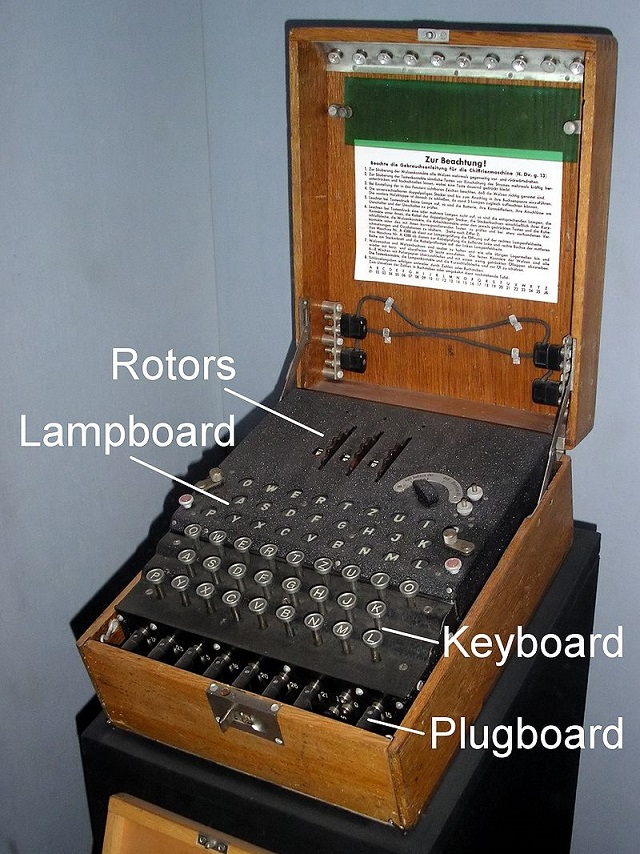
\includegraphics[width=0.5\textwidth]{EnigmaMachineLabeled}
\caption{A Recreated Enigma Machine}
\label{fig:EM}
\end{figure}   

%%%%%%%%%%%%%%%%%%%%%%%%%%%%%%%%%%%%%%%%%%%%%%%%%%%%%%%%%%%%%%%%%%%%%%%%%%%%%%%%
\section{COMPUTER HARDWARE}

The history of computer hardware started in the 1960. The focalpoint was the  
vacuum tubes turned to solid-state devices such as the transistor and later 
the integrated circuit. By 1959 discrete transistors were considered 
sufficient, reliable, and economical that they made further vacuum tubes 
obsolete and uncompetitive. Computer memory slowly moved away from 
magnetic core memory devices to solidstate static and dynamic semiconductor and
memory, which greatly reduced the cost, size and power usage of 
computers.Colossus was the world's first electronic digital programmable 
computer. It used a large number vacuum tubes. It had papertape 
input and was capable of being configured to perform a variety of boolean 
logical operations on its data. However, it was not Turing complete.TRADIC was 
the first transistor computer. TRADIC known as Transistor DIgital Computer or 
TRansistorized Airborne DIgital Computer was an all transistorized computer. 
It was the US that completed it in 1954. The computer was built by Jean Howard 
Felker of Bell Labs for the United States Air Force. 

\section{COMPUTER SOFTWARE}
Since the requirements of these early computers were 
awfully specific, they did not have software developed 
for them, and the instructions that a computer would follow 
was purely dependent on its mechanical features. 
This changed with Manchester Mark I, which featured the 
very first stored program, giving rise to the development 
of software. By creating instructions in the form of computer 
memory, multiple processes could be performed by a single 
computer, and those processes could become even more complex 
with a fraction of the setup time.

\section{CONCLUSION}

In conclusion, the invention of the computer was to make computations faster. Before computers, people had to do calculations using punchcards and calculators. This process was long and tiring so innovators around the world looked for ways to make computations easier. During World War II, the demand and desperation for faster easier computations increased. This gave incentive for increasing funding and research into making calculating faster, which eventually led to the birth of the computer. Without the birth of the computer, technology would not be as advanced as it is today. It made lives easier and helped science and technology grow exponentially. 

\section*{REFERENCES}
References.

\begin{enumerate}[label={[\arabic*]}]
\item Figure 1 image sourced from Wikipedia
\item Martin Campbell-Kelly, John Gustafson, 
Brian Randall, Horst Zuse, (2011, January),
Revolution [Online]. Available E-Mail:
For E-mail, see https://computerhistory.org/contact-us/.
\end{enumerate}

\end{document}
